\documentclass[12pt]{article}

\usepackage{latex/ediArticle}  %from ediArticle.sty
\usepackage{amsmath}

% Settings for the author block
\usepackage{authblk}
\usepackage{ragged2e}
%%%%%%%%%%%%%%%%%%%%%%%%%%%%%%%%%%%%%%%%%%%%%%

% left align title, authors, and affiliations
\makeatletter
\renewcommand\maketitle{\par
  \begingroup
    \flushleft
    \LARGE \setstretch{1.1} {\@title}\par
  \endgroup
  \vspace{-0.2em}
  \begin{flushleft}
    \normalsize \setstretch{1.1} \@author
  \end{flushleft}
}
\makeatother
\renewcommand\Affilfont{\small \itshape}

\title{Burden and health-related quality of life among caregivers of people with motor neuron disease}
\author[1,*]{FirstName LastName}
\author[1,2]{FirstName LastName}
\affil[1]{Affiliation, Department, City, Country}
\affil[2]{Affiliation, Department, City, Country}

\affil[*]{Corresponding author: name.surname@email.edu}

%\affil[*]{corresponding.author@email.example}
%\affil[+]{these authors contributed equally to this work}

%\author{First Author Name$^{a}$$^{*}$, Second Author Name$^{b}$$^{c}$, etc.$^{a}$$^{c}$ \\
%        \small $^{a}$ Department, University, City, Country \\
%        \small $^{b}$Department, University, City, Country \\
%        \small $^{c}$Department, University, City, Country \\
%        \small $^{*}$Corresponding author: email.address \\
%}
\date{}

\begin{document}


% Set font size to 13pt
\fontsize{13pt}{15pt}\selectfont

\maketitle

%\begin{abstract}
%Example Abstract. Abstract must not include subheadings or citations. Example Abstract. Abstract must not include subheadings or citations. Example Abstract. Abstract must not include subheadings or citations. Example Abstract. Abstract must not include subheadings or citations. Example Abstract. Abstract must not include subheadings or citations. Example Abstract. Abstract must not include subheadings or citations. Example Abstract. Abstract must not include subheadings or citations. Example Abstract. Abstract must not include subheadings or citations.
%\end{abstract}

% Which is better in predicting impact on caregivers
% RQ - Determinants of carers impact based on ZBI and HRQoL
% Impact of resource use on the carer and the patient

\section*{Introduction} %%%%%%%%%%%%%%%%%%%%%%%%%%%%%%
Pending
%Motor neuron disease (MND) is a progressive neurodegenerative disease that impacts not only patients but also their informal caregivers. Several studies on ALS in Australia \parencite{lillo_caregiver_2012}, United States \parencite{qutub_life_2014, burke_caregiver_2015, roach_dynamics_2009}, Turkey \parencite{tulek_care_2023}, Ireland \parencite{galvin_caregiving_2016}, Germany \parencite{schischlevskij_informal_2021}, and China \parencite{geng_patients_2017}, have investigated the factors contributing to caregiver burden in ALS and the associated impact of caregiving on the quality of life of these individuals. \textcite{lillo_caregiver_2012} found that patients' abnormal behavior and caregiver stress were the strongest predictors of high caregiver burden, while physical disability was not significantly associated. 

%A cross-sectional study of 33 patient-caregiver pairs, which showed that high caregiver burden was associated with greater patient apathy, disinhibition, and executive dysfunction, as well as caregiver distress \parencite{burke_caregiver_2015}. \textcite{qutub_life_2014} study also found that patients' functional status did not affect caregivers' burden. \textcite{schischlevskij_informal_2021} results showed that caregiver burden increased with patients' decline in functional status - patients' wheelchair use and need for supervision were the strongest predictors of burden.

%\textcite{tulek_care_2023} study corroborates sex as having a significant relationship to caregivers' burden. \textcite{geng_patients_2017} found an association between caregiver burden and older caregiver age. Other factors related to caregivers' burden are difficulties in managing ALS, the emotional or psychosocial impact of caregiving, limitations or restrictions, and the effects on relationships that caregiving has on the caregivers \parencite{galvin_caregiving_2016}. Patients' functional status affect caregiver quality of life \parencite{roach_dynamics_2009}.

\section*{Methods} %%%%%%%%%%%%%%%%%%%%%%%%%%%%%%

\subsection*{Study design and participants}
COMMEND was a randomized controlled trial designed to assess whether a psychological therapy, acceptance and Commitment therapy, was effective for improving quality of life in people with motor neuron disease \parencite{gould_randomised_2022}. Patients with a definitive or probable diagnosis of MND were enrolled from 14 UK MND Care clinics and through self-referral. The study also recruited informal caregivers of people with MND, but absence of a participating caregiver will not preclude a person with MND taking part in the trial. Data were collected for patients and caregivers at  baseline, 6 months, and 9 months. Full details of the baseline patient and caregiver demographics and characteristics, including comorbidities and medications used, have been reported previously \parencite{gould_acceptance_2024, keetharuth_costeffectiveness_2024}. The present study focuses on the caregivers. 

\subsection*{Data and questionnaires}
We assessed caregiver burden at every visit using the 22-item version of Zarit Burden Interview (ZBI). ZBI is a widely-used instrument for assessing the perceived burden experienced by caregivers \parencite{zarit_relatives_1980}. The questions cover the caregiver’s health, psychological well-being, finances, social life, and relationship with the patient. The 22-item version of ZBI contains five-point Likert-style questions with responses to each item ranging from 0, denoting “never”, to 4, denoting “nearly always”. \parencite{zarit_hidden_1985}. The total score therefore ranges from 0 to 88, with a higher score indicating a greater perceived care burden. 

Caregivers self-assessed their HRQoL at using the EuroQol Visual Analogue Scale (EQ-VAS) and 5-dimension (EQ-5D) questionnaires \parencite{herdman_development_2011}. For EQ-5D, they scored their current health state in each of five domains (pain/discomfort, anxiety/depression, mobility, usual activities, and self-care) using a 3-point scale (no, moderate, or extreme problems). From the health-state profile obtained, we used mapped tariffs from EQ-5D-5L to EQ-5D-3L \parencite{hernandez_alava_eq-5d-5l_2018} to calculate the utility score (EQ-5D index score), ranging between 0 (represents death) and 1.0 (represents perfect health). Caregivers rated their current health status on the day of assessment using EQ-VAS, which ranges from 0 (worst imaginable health) to 100 (best possible health). The mean norm value in the English population is reportedly XX (\textbf{REF}). 

Factors related to the informal caregivers and patients were collected at baseline (\autoref{tab_var_category}). These included age,sex, educational level, work status, change in work status, relation to the patient with ALS, and whether cohabiting with the patient, was collected at baseline.  We also asked respondents if they had any medical conditions. Other variables were caregiving context, including relationship with care recipient, intensity of caregiving activities, and how long has been looking after. The information information on characteristics of patients with ALS (\autoref{tab_var_category}) included age, sex, marital status, employment situation, educational level, presence and number of comorbidities, duration of disease, disease severity. . Disease severity was measured using the ALS Functioning Rating Scale‐Revised, ALSFRS‐R \parencite{cedarbaum_alsfrs-r_1999}. We used the algorithm developed by \textcite{balendra_estimating_2014} to calculate King's clinical stages from ALSFRS-R scores. The King's staging system is based on disease burden and consists of five disease stages (1 to 5) with stage 1 being onset of disease in one anatomical region and stage 5 being death.

\begin{table}[H]
    \centering \singlespacing \small
    \caption{Categorization of independent variables}
    \begin{tabular}{|L{6cm}|L{9cm}|}
        \hline
        \PlainInput{tables/tab_var_category}
    \end{tabular}
    \label{tab_var_category}
    \caption*{\footnotesize \textit{Notes:} Rate of deterioration uses an estimate of the average deterioration in ALSFRS-R score per month between symptom onset and baseline. ALSFRS-R, Revised Amyotrophic Lateral Sclerosis Functional Rating Scale; EQ-5D, EuroQol 5-dimension questionnaire; HADS, Hospital Anxiety and Depression Scale; MQOL, McGill Quality of Life Questionnaire}
\end{table}

\subsection*{Statistical analysis}
We described the characteristics of the participants (patients with MND and caregivers) using means and standard deviations for continuous variables and using numbers and percentages for categorical variables. We then assessed the impact of patient’s functional status on caregivers using analysis of variance (ANOVA). For this analysis, data from all caregivers at all time points (baseline, 6 months, and 9 months) were pooled. The caregiver EQ-5D and ZBI were compared using t-tests for the differences between baseline, and 6 months, and 9 months. We used Spearman coefficients to assess correlations between caregiver burden and quality of life scores between baseline and 9 months.Lastly, we conducted multiple regression analyses to test the extent to which caregiver- and patient-related variables explained caregiver burden and HRQoL.
To select independent variables for the model. we did a series of univariate linear regression to examine the direction and size of the relationships between caregiver burden and possible influencing factors on  caregivers’ burden (ZBI) and health-related quality of life (EQ-5D). We selected variables to add to multiple linear regression by adopting a critical level of significance (p $\leq$ 0.05) in the univariate analysis. All caregiver background characteristics were included regardless of significance.
All analysis were conducted using Stata version 18.0 (StataCorp, College Station, Texas, USA).

\section*{Results} %%%%%%%%%%%%%%%%%%%%%%%%%%%%%%
At baseline, the study cohort analyzed comprised 93 caregivers that consent was obtained to participate in the study, alongside the patients in their care. Both ZBI and HRQoL data at was collected from a total of 86 caregivers at baseline, of which 85 had complete and data on all outcome measures. One caregiver-patient pair was were excluded from further analyses because the EQ-5D score was negative while the VAS score was 100, resulting in 84 full observations. %This represents about 1.5\% of an estimated 5700 patients (prevalence, 8.6 per 100,000 persons) that lived with MND in 2020 \textbf{10.1080/21678421.2019.1587629}. The total number of caregivers with available data at the 9-month timepoint (and for the change from baseline to 9 months was) was: ZBI, n = 66; EQ-5D, n = 67.

\subsection*{Caregiver and patient characteristics}
\autoref{tab_desc_stat} summarizes the baseline sociodemographic and clinical characteristics of the caregivers and patients. Caregivers had a mean (SD) age of 59.7 (11.8) years and most (70.2\%) caregivers were female, consistent with previous literature \parencite{schischlevskij_informal_2021}. Approximately half of the caregivers (4.8\%) reported being in paid employment.  Most caregivers (92.9\%) were direct family members of the patients and likely living together with a partner with MND as observed in previous studies \parencite{burke_longitudinal_2018, galvin_caregiving_2016, schischlevskij_informal_2021}. The median duration of caregiving (DOC) was three hours per day (as stated by the main CG; additional hours by more than one CG per patient are possible).  The mean ZBI scores at baseline was 21.1 (12.3). The EQ-VAS mean (79.8/100) was the same as the estimated EQ-5D-5L index score with 0.80/1. These HRQoL values were slightly lower than that in the general British population (EQ-5D score value for a 62 year old: male, 0.82; female; 0.84) \parencite{hernandez_alava_estimating_2022}.  

Patients had a mean (SD) age of 62.2 (10.6) years, the mean (SD) time since diagnosis was 1.6 (2.9) years, and about half had a physical or mental comorbidity (mean of 0.6 comorbidities). The mean ALSFRS-R score was 35.5/48 (a score of 48 represents an absence symptoms while 0 represents the worst functional status). The cohort included patients in all disease severity stages, but only 6\% were in King's stage 4. In summary, these characteristics mean that our cohort was relatively younger and had less severe disease compared to previous studies [REF]. 40.5\% of patients were female, consistent with literature that MND diagnosis was more common in men \parencite{burchardt_analysis_2022}.

\begin{table}[H]
    \centering \singlespacing \small
    \caption{Patients’ and caregivers characteristics, patients' functional status (ALSFRS-R), caregiver burden (ZBI score), and caregiver health-related quality of life (EQ-5D) at baseline}
    \begin{tabular}{|L{5cm}|R{3.2cm}|}
        \hline
        \PlainInput{tables/tab_desc_stat}
    \end{tabular}
    \label{tab_desc_stat}
    \caption*{\footnotesize \textit{Notes:} Data are based on participants with non-missing baseline caregiver burden and quality of life data. ALSFRS-R, Revised Amyotrophic Lateral Sclerosis Functional Rating Scale; EQ-5D, EuroQol 5-dimension questionnaire; n, number; SD, standard deviation, VAS, visual analog scale; ZBI, Zarit Burden Interview.
}
\end{table}

\subsection*{Impact of patient's functional status on caregivers}
The mean ZBI score by King's stage showed that caregivers patients with worse functional status had a greater burden, but results were not consistent. \autoref{fig:outcome-kings-stage} shows the ZBI score by King's stage at baseline, 6 months, and 9 months. The ZBI score was highest for carers of stage 4 patients, but higher for stage 2 compared to stage 3. Using baseline data only, scores were < 20 for stage 1/2 and >20 for stage 3/4. We found a weak, negative, correlation between the ZBI score and the ALSFRS-R ($\rho$ = −0.208, p < 0.002). Due to this inconsistency, we use ALSFRS-R instead of King's stages as a measure of patient's functional status for subsequent statistical analyses.

\begin{figure}[H]
    \centering
    \includegraphics[width=1\linewidth]{output/figures/outcome-als-frs.png}
    \caption{Scatter plots of EQ-5D-5L utility scores, domain scores and scores versus ALSFRS-R score at baseline, 6 months, and 9 months}
    \label{fig:dummy}
    \caption*{\footnotesize \textit{Notes:} }
\end{figure}

Using ANOVA on pooled data, we observed statistically significant differences in the mean EQ-5D index scores between the King’s Stages (p = 0.001, \autoref{tab_outcomes_kings}). This finding was supported by a weak, but positive, correlation between the EQ-5D index score and the ALSFRS-R ($\rho$ = 0.216, p = 0.002). Together, these imply that a better (worse) patient’s functional status is associated with led to a higher (lower) caregiver HRQoL. There was no significant association between functional status and either the mobility or self-care, suggesting that these EQ-5D domains were less useful. Similar non-significant results were observed for EQ-VAS scores (p = 0.999)

\subsection*{Caregiver HRQoL and burden over time}
We found significant differences in ZBI scores between 0 and 9  months (mean difference -6.4, <0.001), mostly driven by the change in scores between 0 and 6 months (\autoref{tab_outcomes_time}). There was no meaningful difference between baseline and 9 months in caregiver EQ-5D index score (mean difference 0.02, p-value <0.170) and the caregiver EQ-5D VAS score (mean difference -0.84, p-value <0.743). When we examined the EQ-5D domain scores (\autoref{fig:eq5d-domains-time}), most caregivers did not have serious problems (<5\% for any domain) and no caregiver had extreme problems at baseline and at or other time points. At baseline, no caregiver had any problem in self-care domain. At 9 months, more caregivers had some problems in the domains of pain/discomfort and anxiety/depression compared to other EQ-5D domains.

\begin{table}[H]
    \centering \singlespacing \small
    \caption{Means differences (95\% confidence intervals) and p-values from t-tests comparing of caregiver ZBI, EQ-VAS, and EQ-5D scores changes over time}
    \begin{tabular}{|L{6cm}|C{5cm}|C{2.5cm}|}
        \hline
        \PlainInput{tables/tab_outcomes_time}
    \end{tabular}
    \label{tab_outcomes_time}
    \caption*{\footnotesize 
                \textit{Notes:} CI, confidence interval; EQ-5D, EuroQol 5-dimension questionnaire; VAS, visual analog scale; ZBI, Zarit Burden Interview}
\end{table}

\begin{figure}[H]
    \centering
    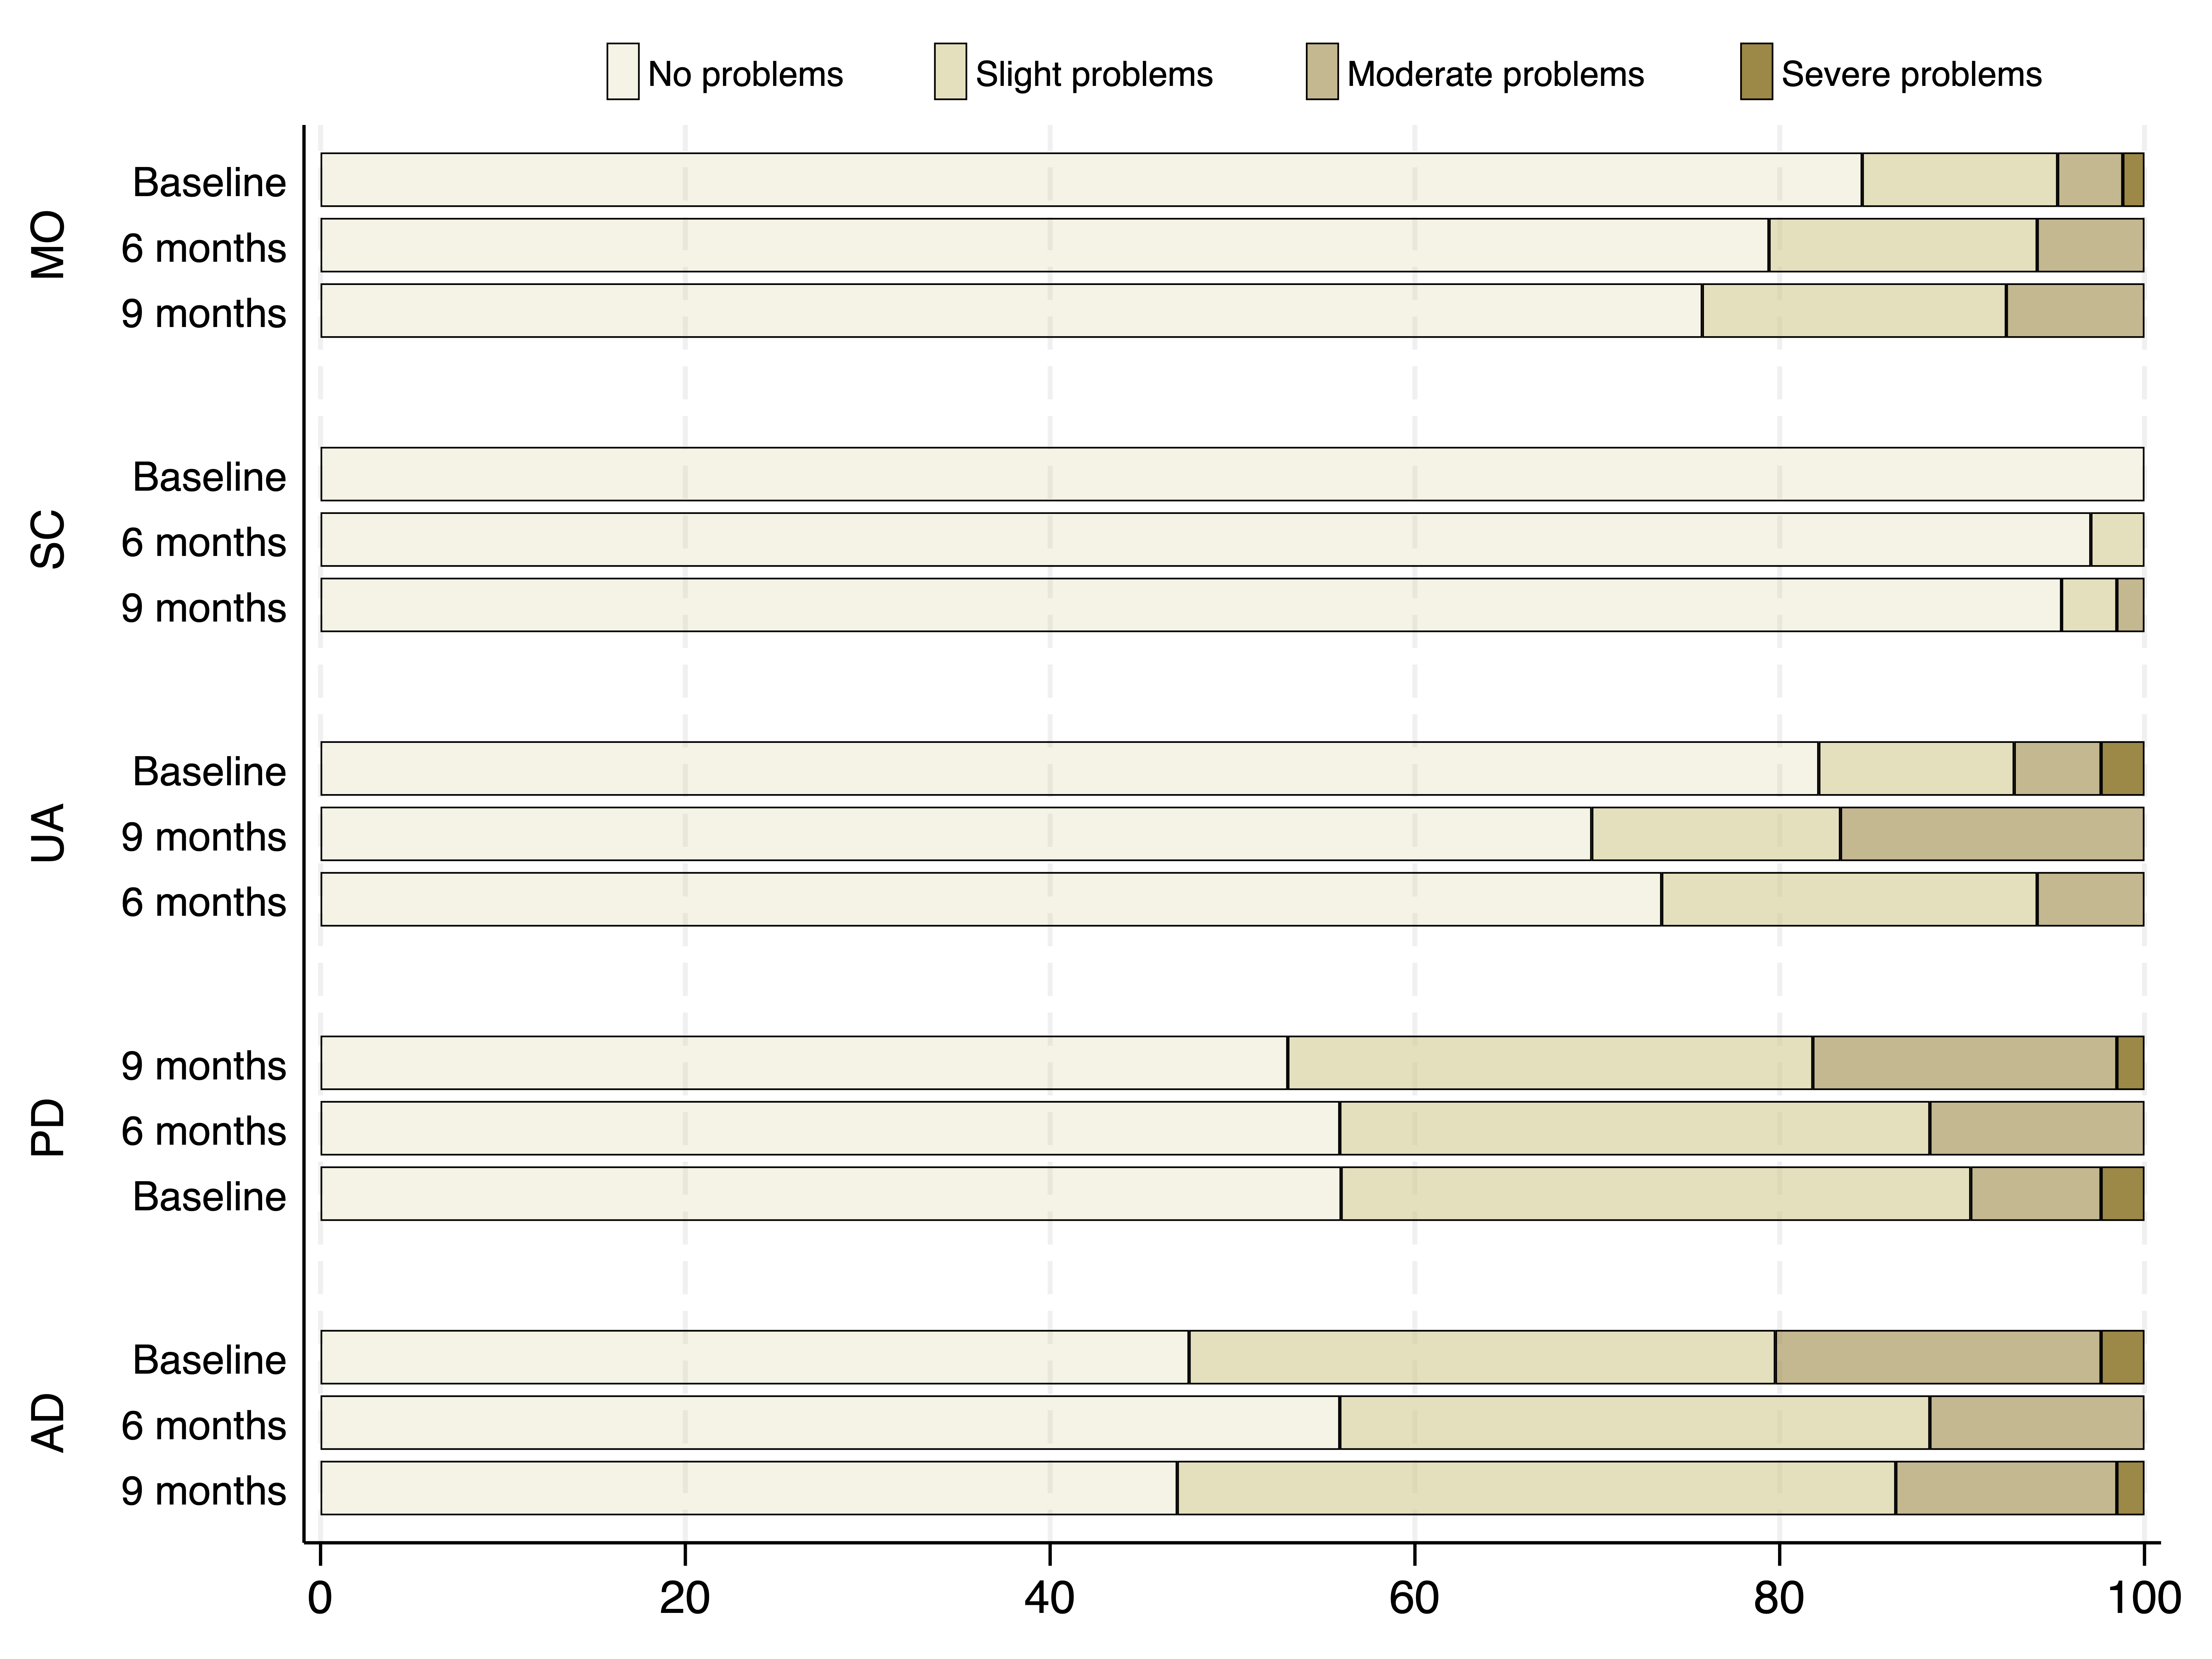
\includegraphics[width=1\linewidth]{figures/eq5d-domains-time.png}
    \caption{Problems in the caregiver EQ-5D domains at baseline, 6 months, and 9 months.}
    \label{fig:eq5d-domains-time}
    \caption*{\footnotesize \textit{Notes:} MO, mobility; SC, self-care; UA, usual activities; PD, pain/depression; AD, anxiety/depression.}
\end{figure}

\subsection*{Relationship between ZBI and EQ-5D}
Correlations were weak or very weak between EQ-5D (index and VAS scores) and ZBI at each time point and for the change scores (\autoref{tab_outcomes_corr}). For the ZBI, the 18-month change score correlation was −0.16 (95\% confidence interval, CI: −0.22, −0.09) for the EQ-5D VAS score and −0.09 (95\% CI: −0.15, −0.03) for the EQ- 5D index score.

\begin{table}[H]
    \centering \singlespacing \small
    \caption{Spearman correlation coefficients between caregiver burden and quality of life scores at baseline, at 9 months, and change in scores between baseline and 9 months.}
    \begin{tabular}{|L{3.6cm}|C{1.7cm}|C{1.4cm}|C{1.7cm}|C{1.4cm}|C{1.7cm}|C{1.4cm}|}
        \hline
        \PlainInput{tables/tab_outcomes_corr}
    \end{tabular}
    \label{tab_outcomes_corr}
    \caption*{\footnotesize 
                \textit{Notes:} EQ-5D, EuroQol 5-dimension; EQ-VAS, EuroQol visual analog scale; ZBI, Zarit Burden Interview}
\end{table}

\subsection*{Factors influencing caregiver burden}

%GOOD WRITE-UP COPIED FROM ANOPTHER PAPER: As already shown above, the patient’s functional status had a clear influence on her/his caregiver’s burden. To provide a deeper analysis of further influencing factors on caregiver burden (ZBI score), multiple regression analysis was used (Table 3). The patient’s wheelchair dependency increased the ZBI score by 9.30 points. Additionally, a rise of 5.01 points was observed, if the patient needed permanent supervision. The main influence on the ZBI appeared to be the CG’s mental health impairment due to caregiving with an increase of 11.36 points. However, physical health impairment had no statistically significant impact on the ZBI score. Furthermore, patients’ age seemed to slightly lower the burden by −0.24 points for each increasing year. Neither the patient’s nor the CG’s gender had statistically significant impacts on the ZBI in the multivariate regression analysis.

\begin{table}[H]
    \centering \singlespacing \small
    \caption{Multivariable OLS regression models of associations between caregiver burden (ZBI) and caregiver- and patient-related independent variables \\
    \textcolor{red}{Model 3 is preferred - explains 20\% of the variance in ZBI scores. Effect disappears if adding patient EQ-5D either as index or the domains. Which model to choose? Could go for Model 3 but between ALSFRS and Patient EQ5D, which is a more relevant predictor?}}
    \begin{tabular}{|L{5cm}|R{1.6cm}|R{1.6cm}|R{1.6cm}|R{1.6cm}|R{1.6cm}|}
        \hline
        \PlainInput{tables/tab_multiOLS_zbi}
    \end{tabular}
    \label{tab_multiOLS_zbi}
    \caption*{\footnotesize 
                \textit{Notes:} ALSFRS-R, Revised Amyotrophic Lateral Sclerosis Functional Rating Scale; MQOL, McGill Quality of Life Questionnaire; ZBI, Zarit Burden Interview}
\end{table}



\begin{table}[H]
    \centering \singlespacing \small
    \caption{Multivariable OLS regression models of associations between health-related quality of life (EQ-5D) and caregiver- and patient-related independent variables \\
    \textcolor{red}{ZBI score is significant and effect persists regardless of controls used. Every one unit increase in ZBI scores (higher numbers mean greater burden) reduces the EQ-5D score by 0.003 points (higher numbers mean better quality of life). All models are similar - explains 12\% of the variance in EQ-5D scores}}
    \begin{tabular}{|L{5cm}|R{1.6cm}|R{1.6cm}|R{1.6cm}|R{1.6cm}|R{1.6cm}|}
        \hline
        \PlainInput{tables/tab_multiOLS_eq5d}
    \end{tabular}
    \label{tab_multiOLS_eq5d}
    \caption*{\footnotesize 
                \textit{Notes:} ALSFRS-R, Revised Amyotrophic Lateral Sclerosis Functional Rating Scale; EQ-5D, EuroQol 5-dimension; MQOL, McGill Quality of Life Questionnaire}
\end{table}


\section*{Discussion} %%%%%%%%%%%%%%%%%%%%%%%%%%%%%%
Pending


\clearpage
\section*{Supplementary Material} %%%%%%%%%%%%%%%%%%%%%%%%%%%%%%

% \renewcommand{\figurename}{Supplementary Figure}
% \setcounter{figure}{0}

\setcounter{table}{0}
\renewcommand{\thetable}{S\arabic{table}}

\setcounter{figure}{0}
\renewcommand{\thefigure}{S\arabic{figure}}


\begin{table}[H]
    \centering \singlespacing \small
    \caption{Pooled carer ZBI, EQ-VAS, and EQ-5D utility and domain scores by King’s stage}
    \begin{tabular}{|L{.33\linewidth}|R{.1\linewidth}|R{.1\linewidth}|R{.1\linewidth}|R{.1\linewidth}|R{.1\linewidth}|}
        \hline
        \PlainInput{tables/tab_outcomes_kings}
    \end{tabular}
    \label{tab_outcomes_kings}
    \caption*{\footnotesize 
                \textit{Notes:} Data from all caregivers at all time points (baseline, 6 months, and 9 months) have been pooled. Comparisons of outcomes between King’s stages use ANOVA. ZBI total score ranges from 0 to 88, with higher scores indicating greater burden. EQ-5D scores range from 0 to 1.0, with higher scores indicating better health-related quality of life. EQ-VAS scores range from 0 to 100, with higher scores indicate better health-related quality of life. EQ-5D domain scores range from 0 to 3, with higher scores indicating greater restriction by domain. \\
                ANOVA, analysis of variance; EQ-5D, EuroQol 5-dimension questionnaire; VAS, visual analog scale; ZBI, Zarit Burden Interview}
\end{table}



\begin{table}[H]
    \centering \singlespacing \small
    \caption{Multivariable Beta regression models of associations between caregiver burden (ZBI) and caregiver- and patient-related independent variables}
    \begin{tabular}{|L{5cm}|R{1.6cm}|R{1.6cm}|R{1.6cm}|R{1.6cm}|R{1.6cm}|}
        \hline
        \PlainInput{tables/tab_multiBeta_zbi}
    \end{tabular}
    \label{tab_multiBeta_zbi}
    \caption*{\footnotesize 
                \textit{Notes:} ALSFRS-R, Revised Amyotrophic Lateral Sclerosis Functional Rating Scale; MQOL, McGill Quality of Life Questionnaire; ZBI, Zarit Burden Interview}
\end{table}



\begin{table}[H]
    \centering \singlespacing \small
    \caption{Univariable OLS regression models of associations, with ZBI as dependent variable, used in selection of independent variables for multivariable regression}
    \begin{tabular}{|L{6cm}|C{2cm}|C{3cm}|C{2cm}|}
        \hline
        \PlainInput{tables/tab_univarReg_zbi}
    \end{tabular}
    \label{tab_univarReg_zbi}
    \caption*{\footnotesize 
                \textit{Notes:} ALSFRS-R, Revised Amyotrophic Lateral Sclerosis Functional Rating Scale; EQ-5D, EuroQol 5-dimension; HADS, Hospital Anxiety and Depression Scale; MQOL, McGill Quality of Life Questionnaire; ZBI, Zarit Burden Interview}
\end{table}



\begin{table}[H]
    \centering \singlespacing \small
    \caption{Univariable OLS regression models of associations, with EQ-5D as dependent variable, used in selection of independent variables for multivariable regression}
    \begin{tabular}{|L{6cm}|C{2cm}|C{3cm}|C{2cm}|}
        \hline
        \PlainInput{tables/tab_univarReg_eq5d}
    \end{tabular}
    \label{tab_univarReg_eq5d}
    \caption*{\footnotesize 
                \textit{Notes:} ALSFRS-R, Revised Amyotrophic Lateral Sclerosis Functional Rating Scale; EQ-5D, EuroQol 5-dimension; HADS, Hospital Anxiety and Depression Scale; MQOL, McGill Quality of Life Questionnaire; ZBI, Zarit Burden Interview}
\end{table}


\begin{figure}[H]
    \centering
    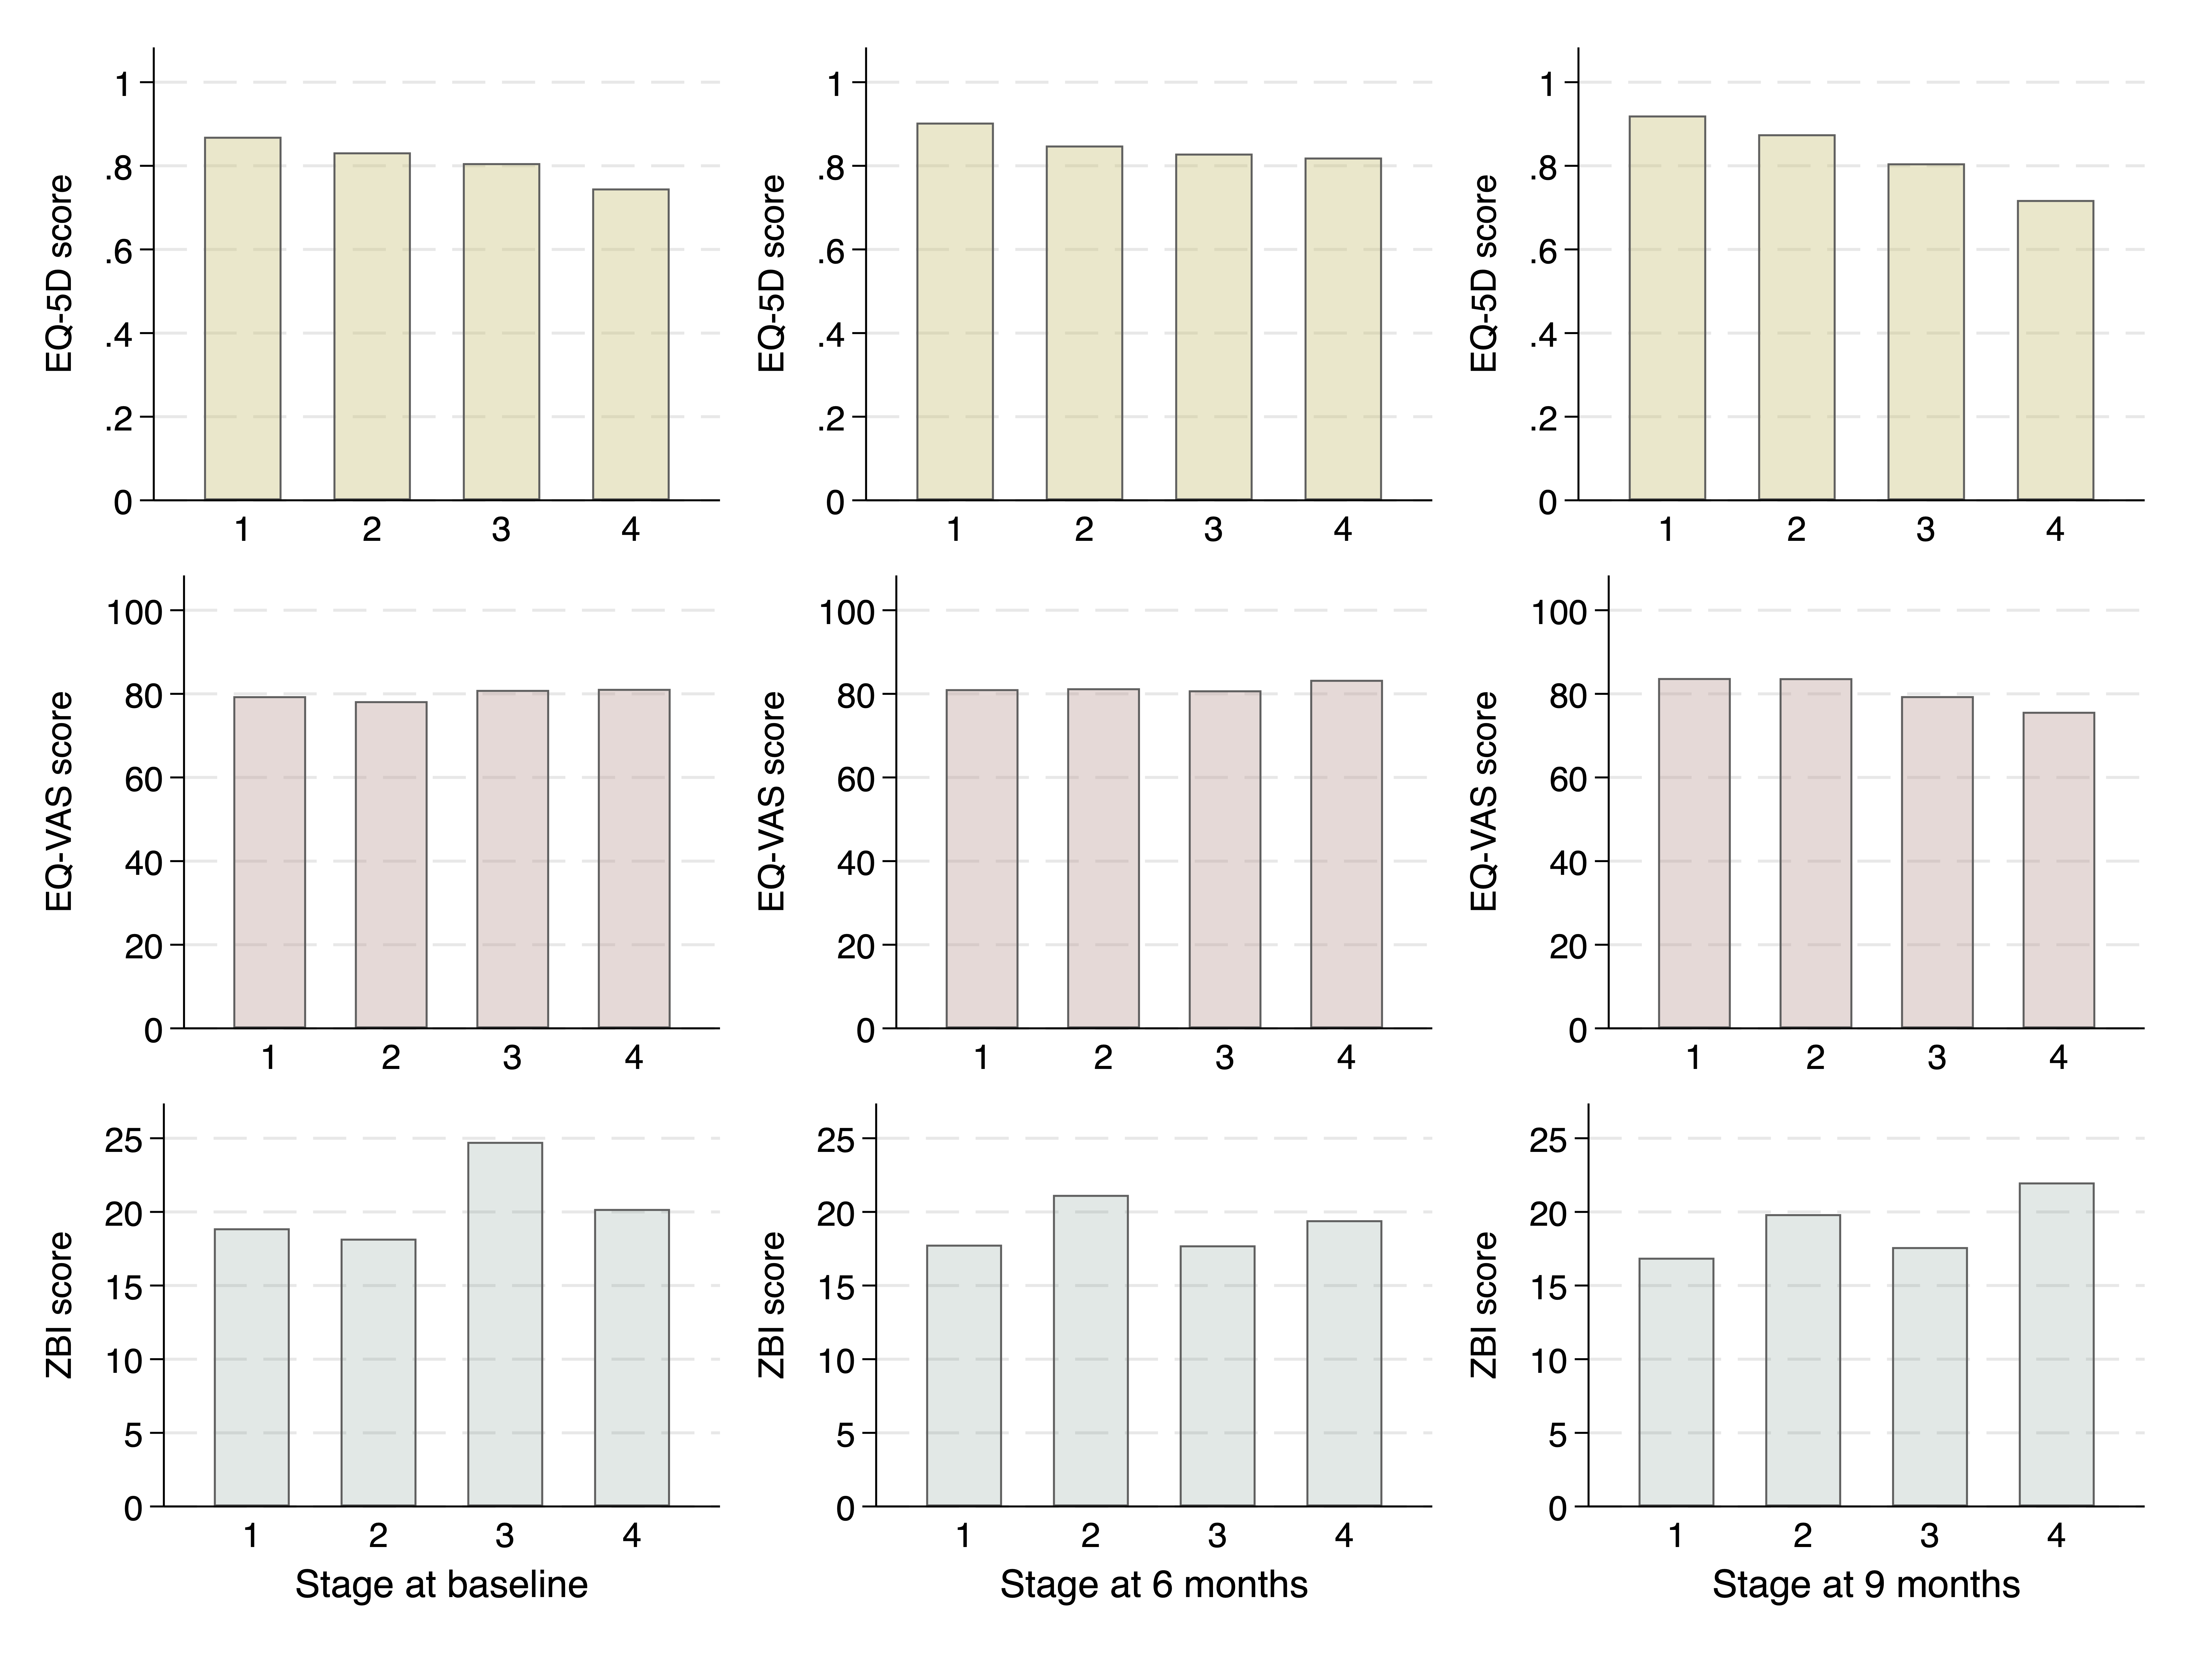
\includegraphics[width=1\linewidth]{figures/outcome-kings-stage.png}
    \caption{EQ-5D-5L utility scores, domain scores and scores by King’s stage}
    \label{fig:outcome-kings-stage}
    \caption*{\footnotesize \textit{Notes:} ANOVA, analysis of variance; EQ-5D, EuroQol 5-dimension questionnaire; VAS, visual analog scale; ZBI, Zarit Burden Interview}
\end{figure}


\begin{figure}[H]
    \centering
    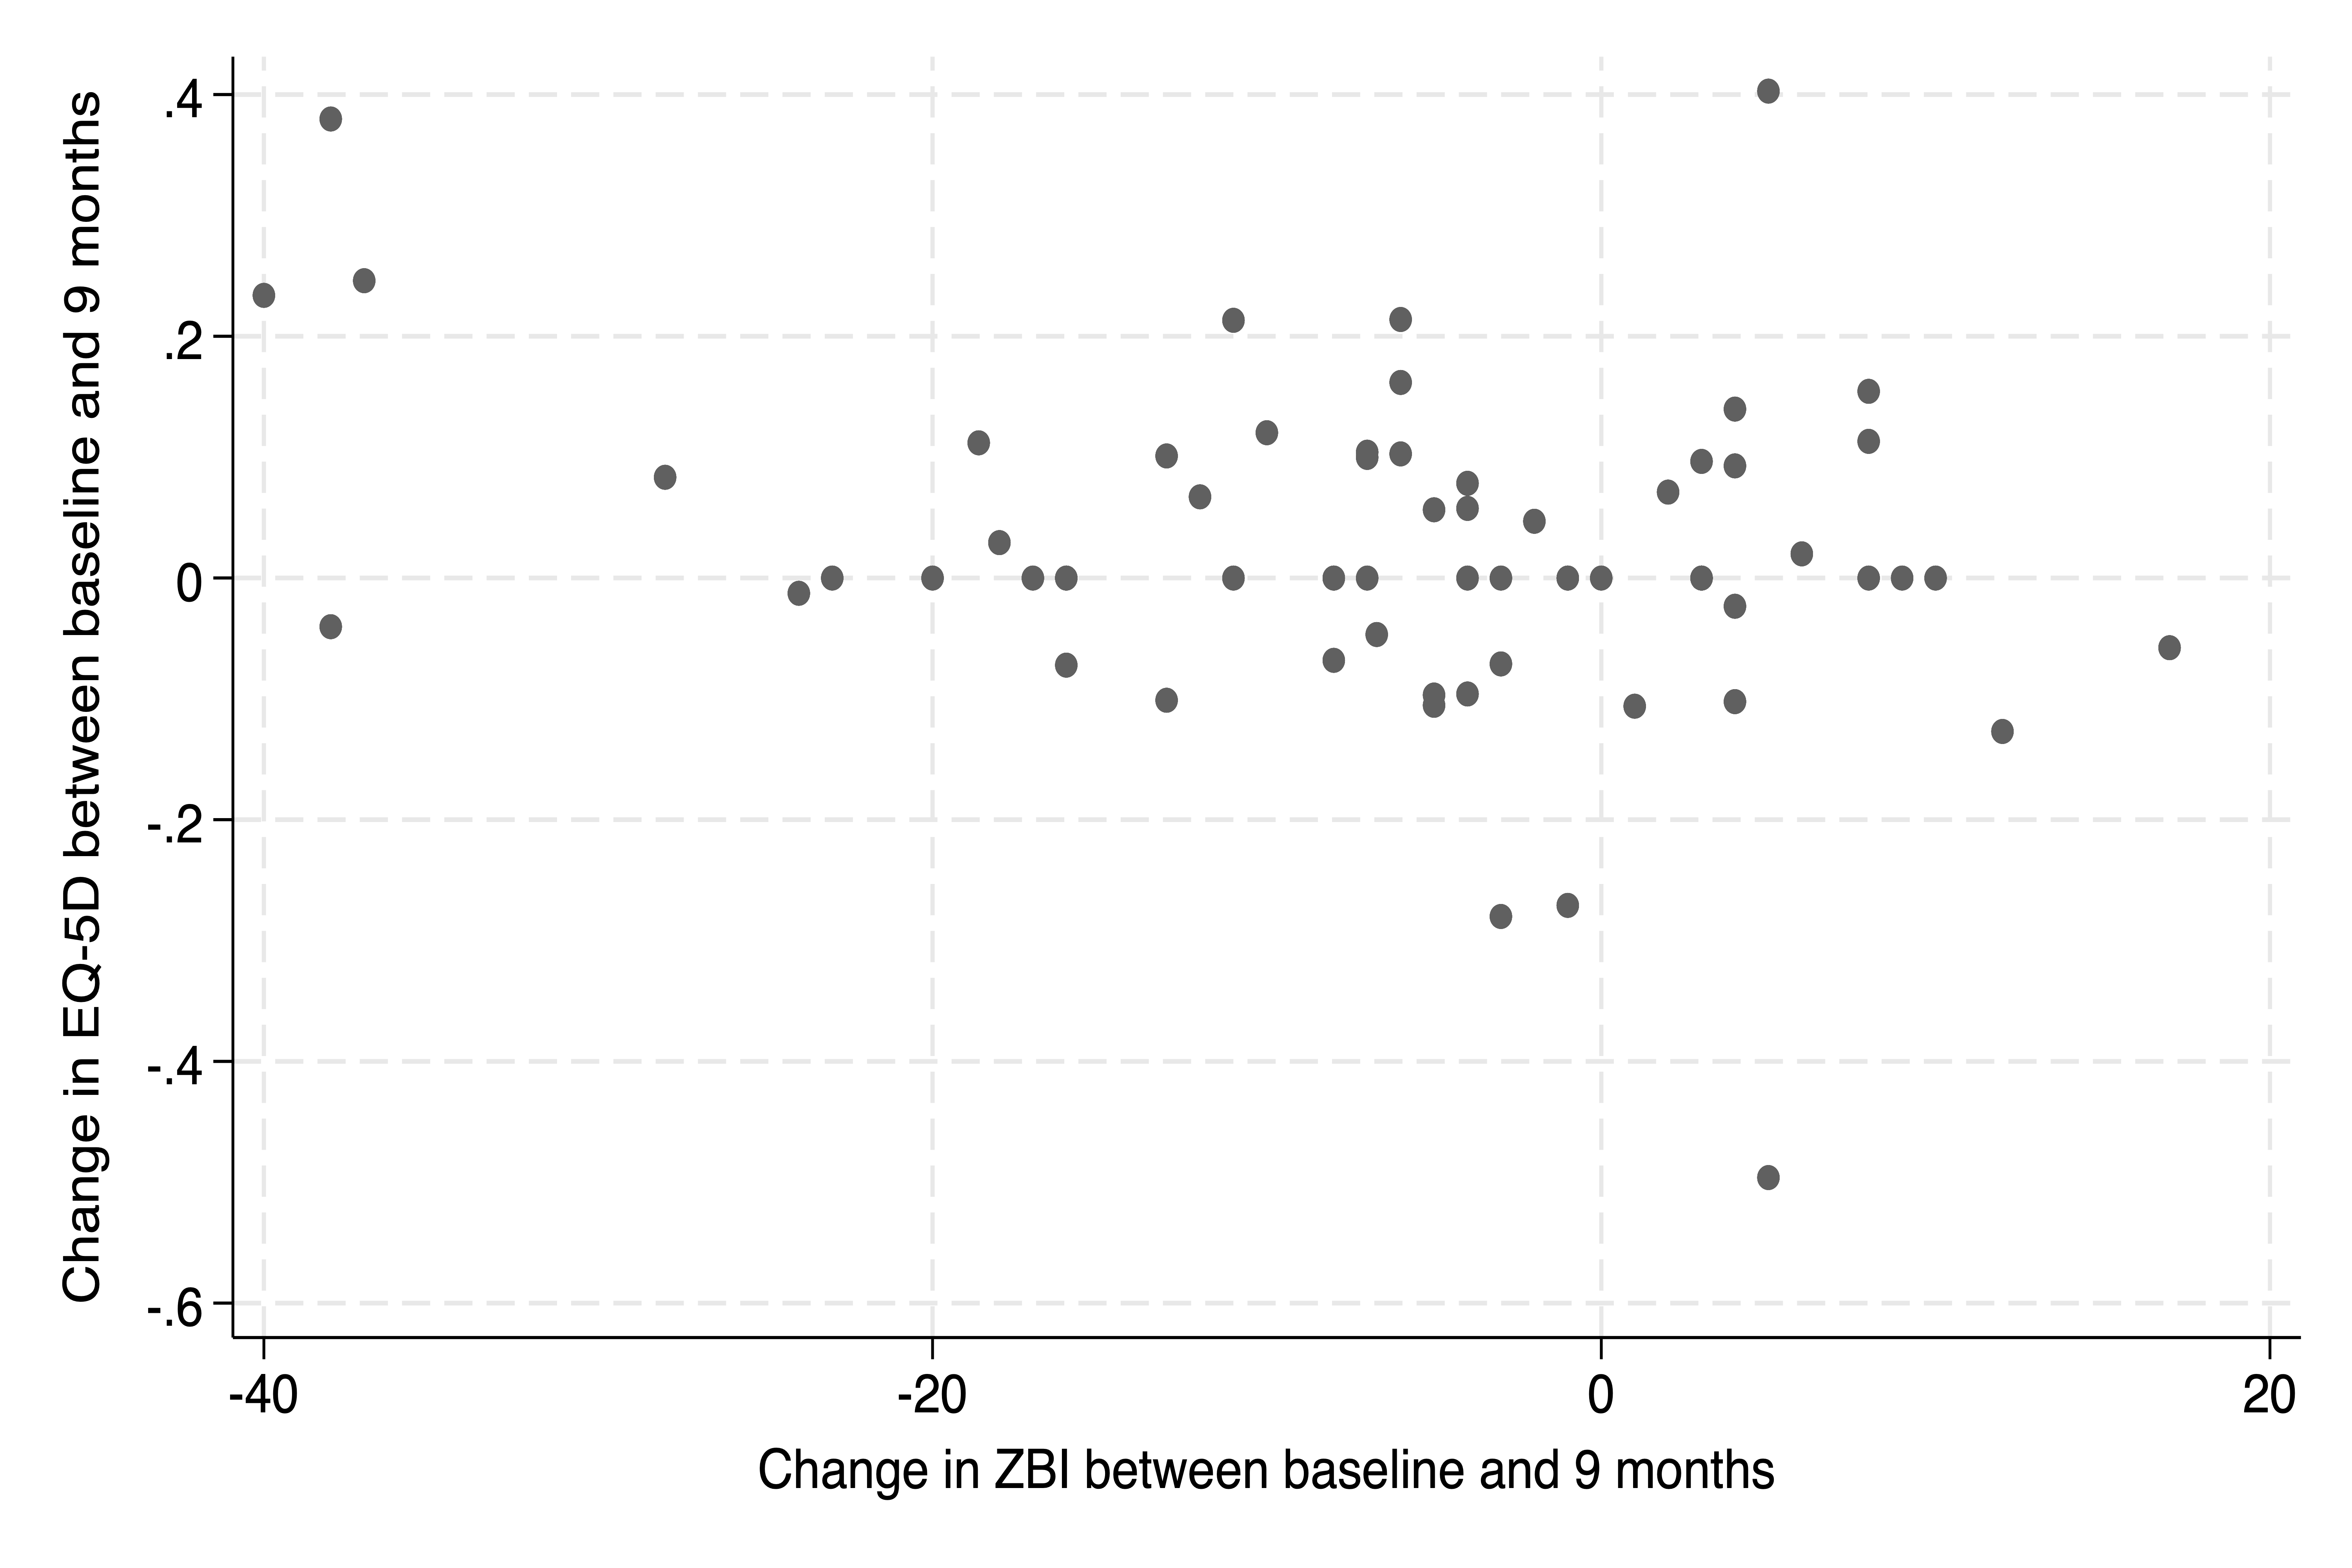
\includegraphics[width=1\linewidth]{output/figures/zarit-eq5d-scoreD.png}
    \caption{Scatter plots showing the relationship between the changes in EQ-5D and change in ZBI between baseline and 9 months of methods reporting and the bibliometric indices. }
    \label{fig:zarit-eq5d-scoreD}
    \caption*{\footnotesize \textit{Notes:} EQ-5D, EuroQol 5-dimension; ZBI, Zarit Burden Interview.}
\end{figure}

\textcolor{red}{\textbf{Comment:} EQ-5D change correlates with ZBI change (\autoref{fig:zarit-eq5d-scoreD}), but no change in EQ-5D over 6- or 9-months! (\autoref{tab_outcomes_time})}

%%%%%%%%%%%%%%%%%%%%%%%%%%%%
%%% %%%
%%% Bibliography %%%

\clearpage
\newrefcontext[sorting=nyt]
\printbibliography


\end{document}